\subsubsection{Sequence Diagram - Module Biểu mẫu}

    Để minh họa chi tiết tương tác giữa các thành phần trong hệ thống, báo cáo trình bày Sequence Diagram đại diện cho luồng xử lý quan trọng trong module Biểu mẫu:
    
    \begin{itemize}
        \item \textbf{Tạo và cấu hình biểu mẫu:} Tương tác giữa người dùng, controller, parser service, S3 storage và database trong quá trình tải lên, phân tích template và cấu hình trường động
    \end{itemize}

    Diagram thể hiện chi tiết các message trao đổi giữa các đối tượng, cơ chế parse file Word để trích xuất placeholder, và cách lưu trữ phân tán giữa S3 (file template) và database (cấu hình trường).

    % ========================================
    % Sequence Diagram - Tạo và cấu hình biểu mẫu
    \newpage
    \begin{figure}[H]
        \centering
        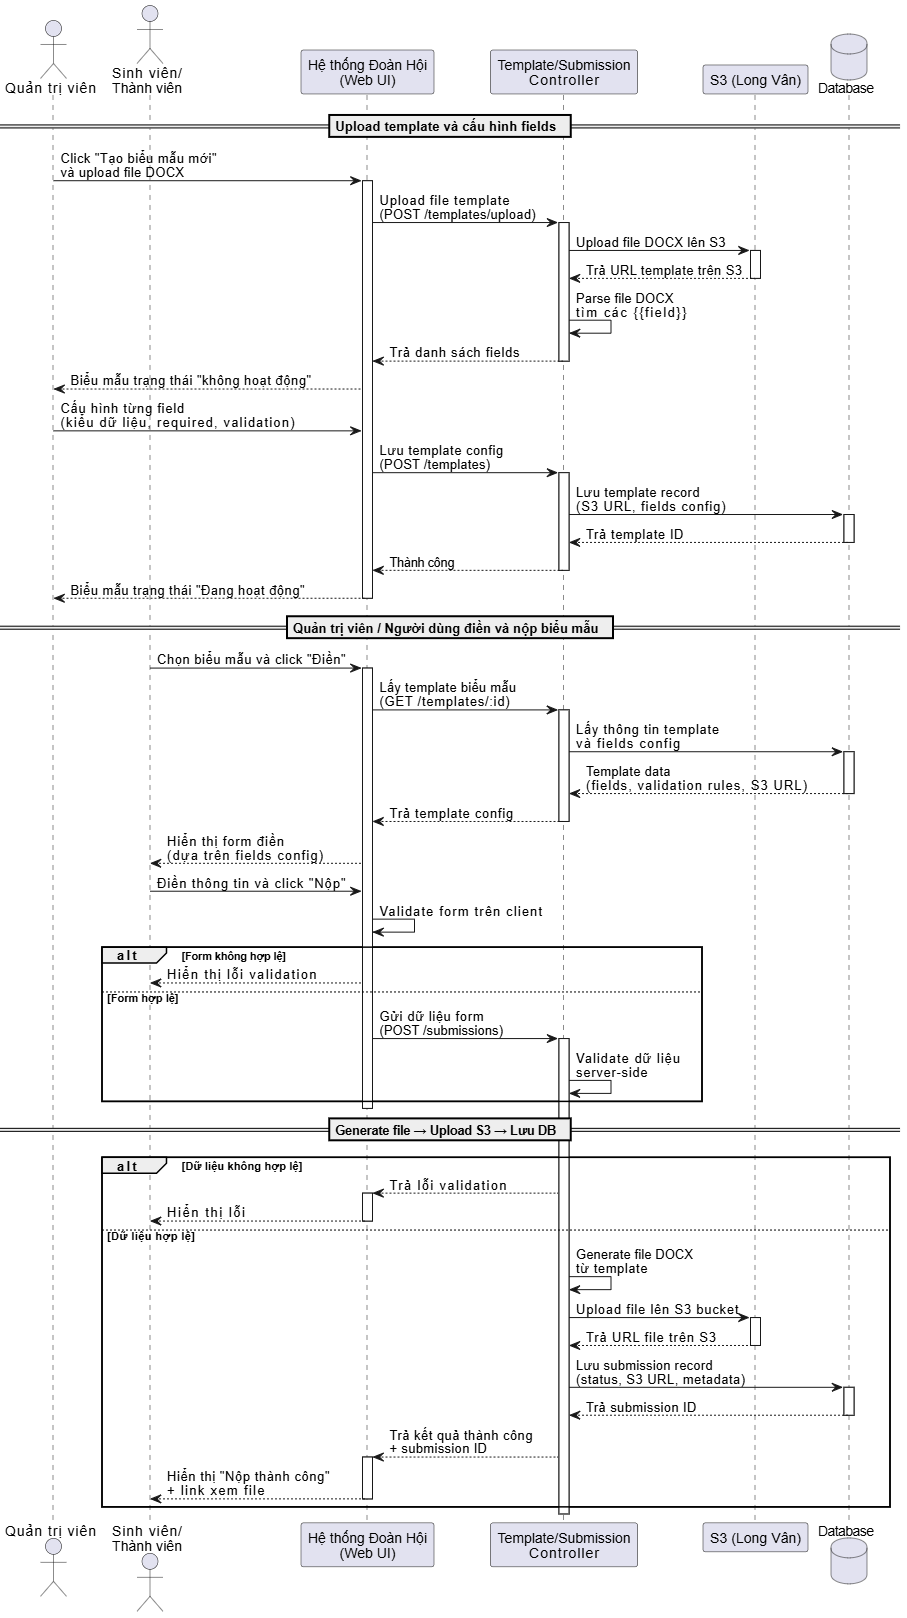
\includegraphics[width=0.8\linewidth]{Images/sequence-diagram/UC08_01_tao_cau_hinh_bieu_mau.png}
        \vspace{0.3em}
        \captionsetup{skip=8pt}
        \caption{Sequence Diagram - Tạo và cấu hình biểu mẫu}
        \label{fig:sequence-uc08-01}
    \end{figure}

    Sequence Diagram trên mô tả tương tác giữa các thành phần khi tạo và cấu hình biểu mẫu động. Actor (Quản trị viên/Người dùng) upload file Word (.docx) qua Controller. Controller validate định dạng file và kích thước (tối đa 5MB), sau đó gọi WordParserService để phân tích nội dung. Parser sử dụng thư viện docx để đọc document structure, tìm kiếm các placeholder theo pattern \{\{field\_name\}\} trong toàn bộ paragraphs và tables. Danh sách placeholder được trả về cho người dùng để cấu hình (nếu không tìm thấy placeholder nào, hiển thị cảnh báo nhưng vẫn cho phép tiếp tục). Người dùng cấu hình từng placeholder: chọn loại dữ liệu, nhập nhãn hiển thị, đánh dấu bắt buộc/tùy chọn. Sau khi hoàn tất, Controller gọi S3StorageService để upload file template lên cloud storage, nhận về URL. Cuối cùng, TemplateService lưu thông tin template (tên, URL S3) và cấu hình trường vào database. Transaction đảm bảo cả file và metadata đều được lưu thành công, nếu có lỗi sẽ rollback và xóa file đã upload trên S3.
